\lstset{language=awk}

\section{Simplex-aðferðin}
Simplex-aðferðin er reiknirit (e. algorithm) sem notað er til þess að leysa línuleg bestunarverkefni.

Notum Wyndor-dæmið (\ref{wyndor:org}) til þess að kynnast aðferðinni
\begin{daemi}
$$\max_{x_1,x_2} z=3x_1+5x_2 $$
m.t.t. skorðanna
\[\begin{array}{ccccc}
 x_1 & && \leq & 4 \\
 & &2x_2 & \leq &12 \\
 3x_1& + &2x_2&\leq&18\\
 &x_1,&x_2&\geq&0
\end{array}\] 
\end{daemi}
Gjaldgegna svæðið er mengi allra punkta sem uppfylla skorðurnar (Sjá mynd \ref{wyndor:img:grafisk}). Ytri mörk skorðanna fást m.þ.a. skipta ójöfnu út fyrir jöfnu. Gjaldgengar hornpunktslausnir, GHL, liggja þar sem ytri mörk tveggja skorða mætast ($m$ skorður í almenna tilfellinu).

Tvær GHL eru sagðar \ath{aðlægar} (e. adjecent) ef þær deila saman einni skorðu ($m-1$ í almenna tilfellinu).

Notum eftirfarandi próf til þess að kanna hvort tiltekin GHL sé besta lausn (e. optimality test):
\begin{setn}[Optimality próf]
 Ef GHL-in hefur aðlægar GHL sem gefa hærra gildi á markfalli (lægra ef lágmörkun) þá er viðkomandi punktur besta lausn.
\end{setn}
\newpage
\subsection{Simplex-aðferðin í grófum dráttum}
\begin{enumerate}
 \item Finna einhverja GHL sem upphafslausn\footnote{Stundum má nota $\vec{0}=(0,\ldots,0)$.}
 \item Ef viðkomandi GHL er besta lausn, þá \emph{hætta}.\label{simplex:gróft}
 \item Færa sig yfir í betri GHL skv.
 \begin{enumerate}[label=(\roman{*})]
  \item Ferðast eftir þeirri skorðu sem gefur \emph{hröðustu aukningu} á markfalli.
  \item Stöðva þegar við rekumst á jaðar lausnarsvæðis.
  \item Finna nýjan punkt m.þ.a. finna skurðpunkt viðkomandi skorða.
 \end{enumerate}
 \item Aftur í skref \ref{simplex:gróft}.
\end{enumerate}

\begin{aths}
 Simplex-aðferðin var uppgötvuð 1947 af G. Dantzig. Hún er enn í fullu gildi -- helstu keppinautar eru innri punkts aðferðir (e. interior point method).
\end{aths}

\section{Viðskeytt form og grunnlausnir}
Gerum ráð fyrir að leysa skuli:
$$\max_{x_1,\ldots,x_n}  z = \sum_{j=1}^n c_j x_j  $$
m.t.t. sk. 
\begin{eqnarray*}
\sum_{j=1}^n a_{ij} x_j  \le  b_i & & i\in\{1,\ldots,m\}\\
x_j  \ge  0, &\quad & j\in\{1, \ldots, n\}
\end{eqnarray*}
þar sem $b_i \ge 0$.

Byrjum með gjaldgengu hornpunktslausninni
$$\vec{x}^{(0)} = \vec{0} \mbox{ þ.e. } x_1^{(0)}=x_1^{(0)}=\ldots=x_n^{(0)}=0$$

Í Simplex-aðferðinni erum við ítrekað að leysa jöfnur þegar farið er úr einni GHL í aðra. Til þess að auðvelda verkið breytum við öllum ójöfnu skorðum í jafnt-og skorður með því að innleiða \ath{slakabreytur} (e. slack variables).
 
Byrjum á að búa til \ath{viðskeytt} (e. augmented) verkefni með aðstoð \ath{slakabreyta} $x_{n+1},\ldots, x_{n+m}$:
$$ \max_{x_1,\ldots,x_n, x_{n+1},\ldots, x_{n+m}}  z = \sum_{j=1}^n c_j x_j  $$
m.t.t. sk.
\begin{eqnarray*}
\sum_{j=1}^n a_{ij} x_j + x_{n+i}  = b_i &\quad& i\in\{1,\ldots,m\}\\
x_k  \ge  0 &&  k\in\{1, \ldots, n+m\}
\end{eqnarray*}

Viðskeytta verkefnið er \emph{jafngilt} því upphaflega þannig að lausn á við\-skeytta verkefninu gefur lausn á upphaflegu verkefninu með því að sleppa slakabreytum. Á fylkjamáli er viðskeytta verkefnið:
$$\max_{\vec{x},\vec{x}_s}  z = \begin{bmatrix}\vec{c}^{T} 
  \vec{0}\end{bmatrix}\begin{bmatrix}\vec{x}\\\vec{x}_s\end{bmatrix}
  = \vec{c_v}^T\vec{x_v} $$
m.t.t. sk.
\begin{eqnarray*}
 \begin{bmatrix}\mat{A} &
  \mat{I}\end{bmatrix}\begin{bmatrix}\vec{x}\\ \vec{x}_s\end{bmatrix} = \mat{A_v}\vec{x_v}  &=&  \vec{b} \\
 \vec{x} \ge  \vec{0}, \vec{x}_s \ge  \vec{0} \mbox{ (eða) }
  \vec{x_v} &\ge& \vec{0}
\end{eqnarray*}
þar sem $\vec{x}$ eru ákvarðanabreytur upphaflega verkefnisins, $\vec{x}_s$ eru slaka\-breytur og $\vec{x}_v$ eru allar ákvarðanabreytur viðskeytta verkefnisins (þ.m.t. slakar).

\begin{daemi}
 Skorðan $x_1\leq4$ er jafngild $x_1+x_s=4$, $x_s\geq0$, þar sem $x_s$ segir til um hversu mikið $x_1$ getur vaxið til þess að skorðan sé bindandi.
\end{daemi}
%Þegar ójöfnuskorðum ($\leq$) hefur verið breytt á þennan hátt segjum við að verkefnið sé á \ath{viðskeyttu formi}.
\begin{daemi}[Wyndor verkefnið \ref{wyndor:org} á viðskeyttu formi]
$$ \max_{x_1,x_2}  z = 3x_1 + 5 x_2 $$
m.t.t. sk. 
\begin{eqnarray*}
 x_1+x_3 & =& 4 \\
 2 x_2 +x_4& =& 12 \\
 3x_1 + 2 x_2 +x_5& =& 18 \\
 x_1 , x_2, x_3,x_4,x_5 &\ge& 0
\end{eqnarray*}
þar sem $x_3,x_4,x_5$ eru slakabreyturnar.
\end{daemi}
\begin{aths}\hspace{.1cm}
 \begin{itemize}
  \item Ef slakabreyta $=0$ þá liggur punkturinn á jaðrinum
  \item Ef slakabreyta $>0$ þá liggur punkturinn innan gjaldgenga svæðisins
  \item Ef slakabreyta $<0$ þá liggur punkturinn utan gjaldgenga svæðisins
 \end{itemize}
\end{aths}


\subsection{Nokkur hugtök}

\begin{itemize}
 \item \ath{Viðskeytt lausn} (e. augmented solution): Gildi á ákvörðana\-breytum, ásamt tilsvarandi gildum á slakabreytum.\footnote{
 Lausnin $\vec{x}=(2,6)$ hefur tilsvarandi viðskeytta lausn \mbox{$\vec{x}_v=(2,6,1,8,5)$}.}
 \item \ath{Grunnlausn} (e. basic solution): Viðskeytt hornpunktslausn.
 \item \ath{Gjaldgeng grunnlausn} (e. basic feasible solution): Viðskeytt GHL.\footnote{
 Lausnin $\vec{x}=(0,6)$ er GHL, tilsvarandi viðskeytt GHL er \mbox{$\vec{x}_v=(0,6,4,0,6)$}.}
\end{itemize}
Fjöldi skorða á viðskeyttu formi er $m$ en fjöldi breyta er $n+m$ (vanákveðið jöfnuhneppi). Getum því valið hvaða gildi sem er á $n$ breytum og leyst fyrir þær sem eftir standa.

Í Simplex-aðferðinni eru þessar breytur settar $=0$ og þær eru sagðar \ath{utan grunns} (e. non-basic variable).
Breyturnar sem eftir standa og við leysum fyrir kallast \ath{grunnbreytur} (e. basic variables).
\begin{verbatim}
 
\end{verbatim}

\subsection*{Samantekt á eiginleikum grunnlausna}
\begin{itemize}
 \item Sérhver breyta er annaðhvort í grunni eða utan grunns.
 \item Fjöldi grunnbreyta er $=m$, fjöldi utan grunns eru $=n$ (og settar $=0)$.
 \item Gildi á grunnbreytum fást m.þ.a. leysa jöfnuhneppi sem samanstanda af skorðum viðskeytts verkefnisins.
 \item Ef grunnbreytur $\geq0$, þá er lausnin gjaldgeng grunnlausn.
\end{itemize}

\section{Algebruleg lausnaraðferð á dæmi}
\begin{daemi}[Lausn á Wyndor Glass Company í \ref{wyndor:org}]
$$ \max_{x_1,x_2}  z = 3x_1 + 5 x_2 $$
m.t.t. sk. 
\begin{eqnarray*}
 x_1 + x_3 & = &4 \\
 2x_2 + x_4 & = &12 \\
 3x_1 + 2x_2 + x_5 & = &18 \\
 x_1,x_2,x_3,x_4,x_5  &\ge& 0
\end{eqnarray*}
\end{daemi}
\begin{lausn}[Algebruleg lausnaraðferð]
\begin{verbatim}
 
\end{verbatim}

\begin{description}
\item[Skref 1] Hér er auðvelt\footnote{Ef við erum með $\le$ skorður og $b$-in eru $\ge 0$ (framboð á hráefni) þá gefur $\vec{x}=\vec{0}$ alltaf löglega lausn.} að finna gjaldgenga hornpunktslausn, setjum $x_1=0$ og $x_2=0$ (þ.e. utan grunns). Í grunni eru slakabreyturnar  með $x_3=4$, $x_4=12$ og $x_5=18$ (lesum beint af skorðunum). Byrjum því með gjaldgengu grunnlausnina $\vec{x}_v=(0,0,4,12,18)$.
 
 
\item[Skref 2] Best væri að framleiða eins mikið og mögulegt er á vöru $x_2$ (vegna þess að
  hagnaðurinn er $5$ og einungis $3$ fyrir vöru $x_1$). Veljum því $x_2$ inn í grunn.

Mesta aukningin fæst m.þ.a. fara eins langt og mögulegt er innan gjaldgenga svæðisins. Gætum að því að þegar $x_2$ vex, þá breytist gildi á öðrum breytum í grunni. Framleiðslan takmarkast af hráefni eða $x_2=6$ og þá þarf slakinn $x_4$ að fara úr $12$ niður í $0$:
\begin{eqnarray}
 x_1 + x_3 & = &4 \nonumber\\
 2 (6) + (0) & = &12 \label{eq:0}\\
 3x_1 + 2 (6) + x_5 & = &18 \nonumber 
\end{eqnarray}
umritum jöfnu \eqref{eq:0}
$$x_2 = \frac{12 - x_4 }{2}$$
og skipum út fyrir $x_2$ í öllum jöfnum og þá fáum við
$$\max_{x_1,x_2}  z = 3x_1 + 5 \frac{12 - x_4}{2} = 30 + 3x_1-\frac{5}{2} x_4$$
\begin{eqnarray*}
 x_1 + x_3 & = &4 \\
 \frac{2 x_2}{2} + \frac{x_4}{2} & = & \frac{12}{2} \\
 3x_1 + 2 \frac{12 - x_4 }{2} + x_5 & =&  18 
\end{eqnarray*}
eða
\begin{eqnarray*}
 x_1 + x_3 & = 4 \\
 x_2 + \frac{1}{2}x_4 & = 6\\
3 x_1-x_4+x_5 &= 6
\end{eqnarray*}
Endum með grunnlausnina $\vec{x}_v=(0,6,4,0,6)$
\item[Skref 3] 
$$\max_{x_1,x_2}  z =  30 + 3x_1-\frac{5}{2} x_4$$
m.t.t. sk.
\begin{eqnarray}
 x_1 + x_3 & = &4 \label{eq:1}\\
 x_2 + \frac{1}{2}x_4 & = &6 \label{eq:2}\\
 3x_1 -x_4 +x_5 & = &6 \label{eq:3}\\
 x_1, x_2, x_3, x_4, x_5 &\ge& 0 \nonumber
\end{eqnarray}
Nú má sjá að við getum grætt á því að framleiða vöru $x_1$
þar sem hagnaðurinn er $3$ en neikvæður fyrir $x_4$. Það mesta
sem við getum framleitt af $x_1$ er fyrir skorður:
\begin{description}
\item[\eqref{eq:1}] $x_1=4$ og $x_3$ lækkar niður í $0$.
\item[\eqref{eq:2}] engar hömlur á $x_1$.
\item[\eqref{eq:3}] $x_1=6/3=2$ og $x_5$ lækkar niður í $0$.
\end{description}
Mesta mögulega \emph{leyfilega} hækkun er því $x_1=2$ og $x_5=0$ (lækkar og fer þ.a.l. úr grunni fyrir $x_1$),
umritum skorðu \eqref{eq:3}:
$$x_1 = \frac{6 + x_4 - x_5}{3}$$
og skiptum út eins og áður:
\begin{eqnarray*}
\max_{x_1,x_2}  z  & = & 30+3\frac{6 + x_4 - x_5}{3} - \frac{5}{2}x_4 \\
 & =& 36-\frac{3}{2}x_4-x_5
\end{eqnarray*}
m.t.t. sk.
\begin{eqnarray*}
 \frac{6 + x_4 - x_5}{3} + x_3 & =& 4 \\
 x_2 + \frac{1}{2}x_4 & =& 6\\
 \frac{3x_1}{3} -\frac{x_4}{3} +\frac{x_5}{3} & = & \frac{6}{3}\\
 x_1, x_2, x_3, x_4, x_5 &\ge& 0 
\end{eqnarray*}
eða
\begin{eqnarray*}
 x_3+\frac{1}{3}x_4 - \frac{1}{3}x_5  & = &2 \\
 x_2 + \frac{1}{2}x_4 & =& 6\\
 x_1 -\frac{1}{3}x_4 +\frac{1}{3}x_5 & =& 2\\
 x_1, x_2, x_3, x_4, x_5 &\ge& 0 
\end{eqnarray*}
Endum með grunnlausnina $\vec{x}_v=(2,6,2,0,0)$
\item[Skref 4] Getum ekki aukið $z$ með því að velja $x_4>0$ eða $x_5>0$ (því stuðlarnir eru neikvæðir). Besta lausn er því fundin, og besta launin á \emph{upprunanlega} verkefninu er $\vec{x}^*=(x_1^*,x_2^*)=(2,6)$ með $z=36$.
\end{description}

\end{lausn}

\section{Simplex-aðferðin á töfluformi}
\ath{Simplex-taflan} er bókhald yfir framgangsmáta Simplex-aðferðarinnar. Hún heldur utan um stuðla í markfalli og skorðum.

Umritum jöfnurnar:
\setcounter{equation}{0}
\begin{eqnarray*}
\max_{x_1,\ldots,x_n} & z - \sum_{j=1}^n c_j
x_j = 0  & (0)\\
\mbox{m.t.t. sk.} & \sum_{j=1}^n a_{ij} x_j + x_{n+i} =  b_i
& (i)\\
\end{eqnarray*}
þar sem $i\in\{1,\ldots,m\}$ og komum þeim fyrir í Simplex-töflu, sjá Töflu \ref{table:simplex}.

\begin{table}[h!]\centering
{
\begin{tabular}{|c|c|c|ccc|ccc|c|}
\hline
grunn- & jafna & $z$ & $x_1$ & $\ldots$ & $x_n$ & $x_{n+1}$ &
$\ldots$ & $x_{n+m}$ & = hægri\\
breytur & & & &$\vec{x}$ & & & $\vec{x}_s$& & ~~~-hlið\\
\hline
 & (0) & $1$ &       & $-\vec{c}^T$ & & 0 & \ldots & 0 & 0 \\
\hline
$x_{1+n}$ & (1) & 0 & & & & & & & \\
$x_{2+n}$ & (2) & 0 & & & & & & & \\
 &  &  & & & & & & & \\
$\vdots$ & $\vdots$ & $\vdots$ & & $\mat{A}$ & & &$\mat{I}$ & & $\vec{b}$ \\
 &  &  & & & & & & & \\
$x_{m+n}$ & ($m$) & 0 & & & & & & & \\
\hline
\end{tabular}}
\caption{Simplex taflan $T$}\label{table:simplex}
\end{table}
 \newpage
\subsection{Aðgerðir á Simplex-töflu}
\begin{aths}G.r.f. að upphaflega verkefnið sé $\max \vec{c}^T\vec{x}$, með skorður $\mat{A}\vec{x}\leq\vec{b}$, $\vec{x}\geq\vec{0}$, og öll $b_i\geq0$. Önnur form LP verkefna eru tekin fyrir í grein \ref{Simplex:onnurform}).\end{aths}
\begin{description}
\item[Upphafsstilling] Koma verkefni yfir á viðskeytt form, slakabreytur í grunni.
 \item[Stoppskilyrði] Athuga hvort besta lausn sé fundin m.þ.a. skoða stuðla við ákvarðana\-breytur í markfalli (lína $(0)$). Ef allir stuðlar $\geq0$, þá er besta lausn fundin. {\bf Hætta}.\label{itrun:simplex}
\item[Finna nýja grunnbreytu] Sú breyta  með stærsta neikvæða stuðlinn í jöfnu (0) (\emph{stærsta} mínus tala í
 efstu línu) er valin, tilsvarandi dálkur kallast \ath{vendidálkur} ($j$). 
\item[Finna grunnbreytu sem fer út] með \emph{minimum ratio test}:
\begin{itemize}
 \item Deila tölum í hægri hlið ($b$-vigur) með tölum úr vendidálki (svo fremur sem þær eru $>0$, ef $=0$ þá sleppt).
 \item Línan með lægsta hlutfallið verður \ath{vendilína} ($i$). Tilsvarandi breyta fer úr grunni.
\end{itemize}
\item[Framkvæma Gauss-eyðingu] til að finna næsta punkt með því að marg\-falda línu með fasta $\neq0$, leggja saman/draga margfeldi einnar línu frá annarri, svokölluð ``elementary row operations''.
\item[Aftur] í stoppskilyrði.
\end{description}

\begin{aths}Ástæða Gauss-eyðingar: Höfum $n$ breytur utan grunns, allar $=0$, \mbox{leysum} $m\times n$ jöfnuhneppi t.þ.a. finna lausnina. Í hverju skrefi Simplex-aðferðarinnar kemur ein ný breyta í grunn og ein fer úr grunni. Gætum leyst jöfnuhneppi frá grunni, en það er óhagkvæmt. Þar sem lítið \mbox{hefur} breyst dugar nokkrar vel-valdar ``elementary row operations'' t.þ.a. finna lausn út frá þeirri gömlu.
 \end{aths}

\subsection*{MATLAB kóði}
\begin{lstlisting}
function T = pivot(T,i,j),
% usage: T = pivot(T,i,j);
  [m, n] = size(T);
  T(i,:) = T(i,:) / T(i,j);
  for k = 1:i-1, T(k,:) = T(k,:) - T(k,j) * T(i,:); end
  for k = i+1:m, T(k,:) = T(k,:) - T(k,j) * T(i,:); end
\end{lstlisting}


\begin{daemi}\label{wyndor:simplex}Beitum töflu-simplex aðferðinni á Wyndor-Glass Company:
\begin{equation}
 \max_{x_1,x_2}  z = 3x_1 + 5 x_2 \nonumber
\end{equation}
m.t.t. sk.
\begin{eqnarray}
 x_1  &\le& 4 \label{eq:4}\\ 
 2 x_2 & \le& 12 \label{eq:5}\\
 3x_1 + 2 x_2 & \le& 18 \label{eq:6}\\
 x_1, x_2 &\ge& 0 \nonumber
\end{eqnarray}
\end{daemi}
\begin{lausn}

Byrjum á því að setja fram líkanið á fylkjamáli:
$$ \max_{\begin{bmatrix}x_1 \\ x_2\end{bmatrix}} z = \begin{bmatrix}3 & 5 \end{bmatrix}\begin{bmatrix}x_1\\x_2\end{bmatrix} $$
m.t.t. sk.
\begin{eqnarray*}
 \begin{bmatrix}1 &  0\\0 & 2\\ 3 & 2\end{bmatrix}\begin{bmatrix}x_1 \\ x_2\end{bmatrix}  &\le&  \begin{bmatrix}4\\12\\18\end{bmatrix} \\
 \begin{bmatrix}x_1 \\ x_2\end{bmatrix} &\ge&  \begin{bmatrix}0 \\ 0\end{bmatrix}
\end{eqnarray*}
\newpage
Tilsvarandi Simplex-tafla er 
\begin{center}
{\renewcommand{\arraystretch}{1.5} \renewcommand{\tabcolsep}{0.2cm}
{\scriptsize
$\begin{array}{|c|ccccc|c|l|} \hline 
 Z &  x_1 &  x_2 &   x_3 &  x_4 &  x_5 &  HH   & \textrm{minratio-test}\\ 
\hline\hline \multicolumn{7}{l}{>> T } \\ \hline 
 1 & -3 & \bf{-5} &  0 &  0 &  0 &  0 & \\
 0 &  1 & 0 &  1 &  0 &  0 &  4 & - \\ 
 0 & 0 & \fbox{\bf{2}} &  0 &  1 &  0 & 12 & 12/2=6 \leftarrow \min \\
 0 &  3 & \bf{2} &  0 &  0 &  1 & 18 & 18/2=9 \\ 
\hline\hline \multicolumn{7}{l}{>> T = pivot(T,3,3)} \\ \hline 
 1 & \bf{-3} & 0 & 0 & \frac{5}{2} & 0 &  30 & \\
 0 & \bf{1} & 0 & 1 &   0 & 0 & 4 & 4/1=4\\
 0 & 0 & 1 & 0 & \frac{1}{2} & 0 & 6 & -\\
 0 & \fbox{\bf{3}} & 0 & 0 & -1 & 1 & 6 & 6/3=2 \leftarrow \min \\
\hline\hline \multicolumn{7}{l}{>> T = pivot(T,4,2)} \\ \hline 
 1 & 0 & 0 & 0 & \frac{3}{2} & 1 &  36 &\\
 0 & 0 & 0 & 1 & \frac{1}{3} & -\frac{1}{3} & 2 &\\
 0 & 0 & 1 & 0 & \frac{1}{2} & 0 & 6 & \\
 0 & 1 & 0 & 0 &  -\frac{1}{3} & \frac{1}{3} & 2 & \\ \hline \hline
\end{array}$
}}\end{center}

%\begin{figure}[b!]
%\centering
%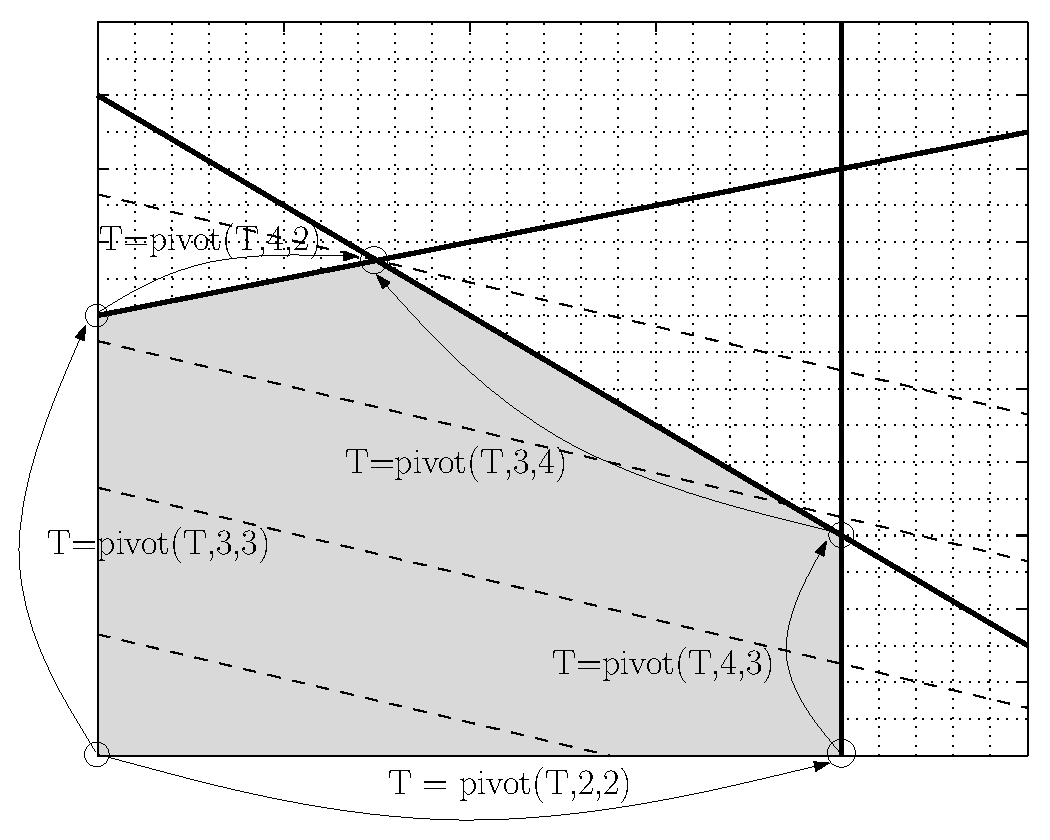
\includegraphics[width=0.9\columnwidth]{figs/daemi_simplex.eps}
%\caption{Rúmfræðileg skýring fyrir simplex-töflu í dæmi \ref{wyndor:simplex}}
%\end{figure}
 
Hér má lesa úr lokatöflunni:
$$\vec{x}_v = (2,~ 6,~ 2,~ 0,~ 0)$$
eða fyrir upprunanlega verkefnið
$$x_1^* = 2 \mbox{ og } x_2^* = 6 \mbox{~~~~~(besta lausn) }$$

Jafnframt er hægt að lesa úr fyrstu línu:
\begin{itemize}
 \item Besta gildi markfallsins: $z^*=36$,
 \item Skuggaverðin (e. shadow prices): $y_1^*, y_2^*, y_3^* = (0,~
\frac{3}{2}, ~ 1)$,
 \item Kostnaðarminnkun (e. reduced costs) fyrir $x_1$ og $x_2$ =
$(0, ~0)$.  
 \item Skorður \eqref{eq:5} og \eqref{eq:6} eru virkar vegna þess að slakabreyturnar $x_4$ og $x_5$ eru ekki grunnbreytur, þ.e.a.s. $x_4=x_5=0$.
\end{itemize}
\end{lausn}

\section{Hvað-ef greining}
Eftir að besta lausn hefur verið fundin er oft mjög gagnlegt að kanna áhrifa þess að breyta stikum líkansins. Slíkt kallast \ath{hvað-ef greining} (e. post\-optimality analysis).

%\subsection{Breytingar á \vec{b}}
Breytingar á hægri hlið skorðu $(i)$, t.d. ef $b_i$ hækkar um 1 þá getur það haft í för með sér breytingu á gildi markfallsins, $y_i=\frac{dz}{db_i}$ sem kallast \ath{skuggaverð} skorðunnar $(i)$.

\begin{daemi}[Hvað-ef greining Wyndor Glass Company]\label{wyndor:postoptimality}
$$\max_{x_1,x_2} z=3x_1+5x_2 $$
m.t.t. skorðanna
\begin{eqnarray}
 x_1 & \leq & 4 =: b_1 \label{postoptimality:1} \\ 
 2x_2 & \leq &12 =: b_2 \label{postoptimality:2} \\
 3x_1 + 2x_2&\leq&18 =: b_3 \label{postoptimality:3}
\end{eqnarray}
Hvaða áhrif hafa breytingar á $\vec{b}=(b_1,b_2,b_3)$ á markfallið?
\end{daemi}
\begin{lausn}
Leysum bestunarverkefnið myndrænt, mynd \ref{wyndor:img:postoptimality}. Sjáum að besta lausn er $\vec{x}^*=(2,6)$, með $z^*=36$.

Þar sem skorða \eqref{postoptimality:1} er ekki virk sjáum strax að ef $b_1$ hækkar um $1$ þá mun það ekki hafa áhrif á gildi markfallsins, því er skuggaverðið er $y_1=\frac{dz}{db_1}=0$.

Aftur á móti, er skorða \eqref{postoptimality:2} virk, svo ef við leyfum $b_2$ að hækka um 1 þá verður hún:
\begin{equation} 2x_2 \leq 13 \label{postoptimality:4}\end{equation}
Leysum nýja skurðpunktinn við skorður \eqref{postoptimality:3} og \eqref{postoptimality:4}, og fáum að nýja besta lausnin yrði $\vec{x}^*=(\frac{5}{3},\frac{13}{2})$ með $z^*=37.5$. Fáum því að breyting um $b_2$ um 1 hefur í för með sér breytingu á markfallinu um $\Delta z=\frac{3}{2}$, því er skuggaverðið er $y_2=\frac{dz}{db_2}=\frac{3}{2}$.

Eins fæst fyrir á breytingu $b_3$ úr 18 í 19 að nýja besta lausnin verður $\vec{x}^*=(\frac{7}{3},6)$ með $z^*=37$. Skuggaverðið er því $y_3=\frac{dz}{db_3}=1$.

\begin{figure}[h!]
\centering
\includegraphics[width=0.8\columnwidth]{figs/wyndor_postoptimality.eps}
\caption{Hvað-ef greining fyrir dæmi \ref{wyndor:postoptimality}}\label{wyndor:img:postoptimality}
\end{figure}
\end{lausn}

\newpage
\section{Samantekt um Simplex aðferðina}
 
\begin{description}
 \item[Z-röðin $(0)$]\begin{verbatim}\end{verbatim}
\begin{itemize}
\item Stuðlar breyta í grunni er alltaf núll.
\item Stuðlar breyta sem ekki eru í grunni geta verið $+$, $-$,
  eða $0$:
\begin{itemize}
\item ef $-$, þá getur breyta komið inn í grunn,
\item ef $+$, þá getur breyta ekki komið í grunn (ef allir stuðla $>0$ þá er
lausnin besta lausn),
\item ef $0$, breyta má koma inn í grunn, en það breytir ekki gildi
markfallsins (ef allir stuðlar eru jákvæðir og a.m.k. einn er núll þá eru
margar bestu lausnir á verkefninu).
\end{itemize}
\item Ef fleiri en ein breyta koma til greina sem næsta breyta í grunn (t.d. markfall $z=3x_1+3x_2$) þá skiptir ekki máli hver er valin.
\end{itemize}
\item[Víkjandi breyta]\begin{verbatim}\end{verbatim}
\begin{itemize}
\item Ef engin breyta getur farið út úr grunni (vendilína) þ.e.a.s. allir stuðlar í þeim vendidálki eru neikvæðir eða núll, þá er vandamálið \ath{ótakmarkað}\footnote{Líklega er villa í framsetningu á bestunarverkefninu, t.d. eina eða fleiri skorður vantar.} (e. unbounded)
\item Ef jafntefli í ``min-ratio'' próf milli tveggja breyta, þá er ein valin af handahófi.\footnote{Í þessu tilviki getur Simplex-aðferðin lent í vand\-ræðum, og farið í ``hringi''. En það kemur sjaldan fyrir í raunveruleikanum.}
\end{itemize}
\item[\ath{Skuggaverð}] (e. shadow price): $y_i = dz / db_i$.
  Skuggaverð fyrir skorðu $i$ mælir breytinguna á markfallinu
  ($z$) sem yrði ef $b_i$ væri aukin.
\item[\ath{Kostnaðarminnkun}] (e. reduced costs) er mesta leyfilega
  aukning í $c_j$ (ef $j$ er ekki grunn breyta) til að halda
  núverandi bestu gjaldgengu grunnlausn, eða m.ö.o. lágmarks hagnaður sem vara $j$ þarf að hækka um til að hún fari í grunn.
\end{description}
\begin{aths}
 Til eru fleiri afbrigði af Simplex-aðferðinni. Munurinn felst í að nota aðrar aðferðir til þess að velja breytu í og úr grunni.
\end{aths}
